% !TeX root=../main.tex

\chapter{روش تحقیق}
در این بخش روش ارائه‌شده را شرح می‌دهیم. در ابتدا تعریفی از مسئله‌ی مورد بررسی در این پژوهش و قیود در نظر گرفته‌شده برای ورودی را بیان می‌کنیم. در ادامه، پیش‌زمینه‌ی محاسباتی راه‌حل استفاده‌شده برای حل مسئله‌ی موردنظر را توضیح می‌دهیم. در انتها الگوریتم پیاده‌سازی‌شده در این روش به صورت مرحله‌به‌مرحله بیان می‌شود.
\section{تعریف مسئله و قیود}
\label{section_problem}
در این پژوهش، ما به دنبال ارائه‌ی یک روش برای حل مسئله‌ی تولید بافت از یک تصویر هستیم، که بر روی الگو‌های تکراری با ساختار پیچیده متمرکز است. برای مشخص کردن مسئله‌ای که به دنبال حل آن هستیم، یک تعریف از مسئله‌ی تولید بافت بیان می‌کنیم:
\begin{definition} \label{texSynProblem}
با استفاده از ورودی یک الگوی دو‌بعدی محدود، خروجی با ساختار یکسان ورودی، ویژگی‌های ظاهری یکسان و به طول و عرض دلخواه تولید شود. 
\end{definition}
این مسئله، یکی از مسائل قدیمی در زمینه‌ی بینایی ماشین بوده که راه‌حل‌های مختلفی با استفاده از روش‌های متفاوت برای آن ارائه‌شده‌است (بخش \ref{texSynLit}). در این پژوهش ما ورودی این مسئله را تنها یک تصویر درنظر می‌گیریم.

ما تلاش می‌کنیم برای طیفی از ورودی‌های خاص، مسئله‌ی \ref{texSynProblem} را حل کنیم. قیود مشخص‌شده برای ورودی، شرایط را برای استفاده از روش مورد نظر ما در حل مسئله فراهم می‌کنند و نتایج تنها برای ورودی‌هایی که این ویژگی‌ها را دارند تولید شده‌است. امکان دارد این روش برای ورودی‌ها با ویژگی‌های متفاوت نیز نتایج مورد قبولی تولید کند یا بتواند برای حل مسائل دیگری استفاده شود، اما این موضوع بررسی نشده ‌است. قیود در نظر گرفته‌شده برای ورودی‌ها در ادامه آمده است:
\begin{itemize}
\item 
الگوی ورودی از تکرار یک قطاع موجود در الگو تشکیل می‌شود.
\item 
تعداد تکرار‌های قطاع در الگو قابل شمارش و محدود است.
\item 
قطاع، ارتفاعی برابر با الگوی اصلی دارد.
\item 
خروجی تنها با استفاده از گسترش افقی تولید می‌شود.
\end{itemize}
\section{پیش‌زمینه محاسباتی} \label{conjGradExp}

در این بخش، الگوریتم \gls{Conjugate Gradient}، که در این روش استفاده می‌شود را شرح داده‌ایم. سیستم معادلات خطی که ماتریس آنها متقارن و مثبت معین است را می‌توان با استفاده از این روش به صورت \gls{Iterative} حل کرد. روش گرادیان مزدوج را می‌توان از دیدگاه‌های مختلف به دست آورد، از جمله روش جهت مزدوج برای بهینه سازی، و تغییر تکرارشونده Arnoldi/Lanczos برای مسائل ارزش ویژه. علیرغم تفاوت در رویکردهای آنها، این روش‌ها یک موضوع مشترک دارند، اثبات متعامد بودن باقیمانده‌ها و مزدوج شدن جهت‌های جستجو. این دو ویژگی برای توسعه‌ی فرمول مختصر روش گرادیان مزدوج بسیار مهم هستند.

می‌گوییم دو بردار غیر صفر u و v با یکدیگر مزدوج هستند (نسبت به \lr{A}) اگر:
\begin{equation} \label{conjGrad1}
	\textrm{u}^T\textrm{Av} = 0
\end{equation}
با توجه به اینکه ماتریس A یک ماتریس متقارن و مثبت‌معین است، قسمت چپ معادله‌ی \ref{conjGrad1} یک ضرب داخلی را مشخص می‌کند:
\begin{equation}
	\textrm{u}^T\textrm{Av} = \langle\textrm{u,v}\rangle_{\textrm{A}} := \langle\textrm{Au,v}\rangle = \langle\textrm{u,A}^T\textrm{v}\rangle = \langle\textrm{u,Av}\rangle
\end{equation}
دو بردار مزدوج هستند اگر و تنها اگر، نسبت به این ضرب داخلی بر هم عمود باشند. مزدوج بودن یک رابطه‌ی متقارن است؛ یعنی اگر u با v مزدوج باشد، v نیز با u مزدوج است.

در نظر می‌گیریم 
\lr{$P=\{\textrm{p}_0, ..., \textrm{p}_n\}$} 
یک مجموعه $n$ عضوی از بردار‌هایی است که دوبه‌دو نسبت به A مزدوج هستند (
\lr{$\textrm{p}_i^T\textrm{Ap}_j = 0$}
، برای هر $i$ نامساوی با $j$). در نتیجه $P$ یک پایه برای فضای برداری 
$\mathbb{R}^n$ 
خواهد بود و ما می‌توانیم پاسخ $x^*$ برای معادله‌ی خطی 
\lr{$\textrm{A}x = \textrm{b}$} 
را با استفاده از این پایه بنویسیم:
\begin{equation}
	x^* = \sum_{i=0}^n\alpha_i \textrm{p}_i \Rightarrow Ax^* = \sum_{i = 0}^{n} \alpha_i \textrm{A}\textrm{p}_i
\end{equation}
اگر دوطرف معادله را از سمت چپ با $\textrm{p}_k^T$ ضرب کنیم، خواهیم داشت:
\begin{equation}
	\textrm{p}_k^T\textrm{b} = \textrm{p}_k^T\textrm{A}x^* = \sum_{i = 0}^{n} \alpha_i \textrm{p}_k^T \textrm{Ap}_i = \sum_{i = 0}^{n} \alpha_i \langle \textrm{p}_k,\textrm{p}_i\rangle_{\textrm{A}} = \alpha_k \langle \textrm{p}_k,\textrm{p}_k \rangle_{\textrm{A}}
\end{equation}
و:
\begin{equation}
	\alpha_k = \frac{\langle \textrm{p}_k, b \rangle}{\langle \textrm{p}_k, \textrm{p}_k \rangle_{\textrm{A}}}
\end{equation}
که با استفاده از این معادله می‌توان ضرایب $x^*$ را در فضای معرفی‌شده به دست آورد. پس باید ابتدا $n$ بردار مزدوج پیدا کرد و سپس ضرایب آن‌ها را برای $x^*$ محاسبه کرد. 

روش بالا، یک روش مستقیم برای حل معادله خطی است که برای $n$ کوچک قابل استفاده است. می‌دانیم در زمینه‌ی تصاویر، مقدار $n$ بزرگ خواهد بود و استفاده از روش بالا بسیار هزینه‌ی بالایی دارد. اگر بردار‌های $\textrm{p}_k$ را با دقت و به درستی انتخاب کنیم، دیگر نیازی به استفاده از تمام این بردارها برای رسیدن به یک جواب مناسب $x^*$ نخواهیم داشت و می‌توانیم با استفاده از روش گرادیان مزدوج، به صورت تکرارشونده، به حل سیستم معادلات خطی بپردازیم. با در نظر گرفتن یک حدس اولیه مانند \lr{$x_0$} (می‌تواند ۰ باشد یا تخمینی از پاسخ نهایی)، در هر تکرار، ما به دنبال پاسخ مناسب خواهیم بود و به یک معیار نیاز داریم تا بدانیم به جواب مناسب، $x^*$، نزدیک می‌شویم یا خیر. این معیار را می‌توانیم با توجه به اینکه $x^*$ به حداقل رساننده‌ی یکتای تابع درجه دوم زیر است، به دست آوریم:
\begin{equation}
	f(x) = \frac{1}{2}x^T\textrm{A}x - x^T\textrm{b}
\end{equation}
وجود یک نقطه‌ی حداقل یکتا برای این تابع، با توجه به متقارن و مثبت معین بودن ماتریس هسین این تابع مشخص است، چون می‌دانیم ماتریس A این ویژگی را دارد و $\textrm{H}(f(x)) = \textrm{A}$. از طرف دیگر می‌دانیم در صورتی که $x^*$ یک نقطه‌ی حداقل‌کننده باشد، باید مشتق تابع را صفر کند. با توجه به اینکه 
$\nabla f(x) = \textrm{A}x - b$ 
در نتیجه این نقطه پاسخ سیستم معادلات خطی نیز خواهد بود.

با توجه به ویژگی‌های گفته‌شده، مناسب است بردار اول پایه
 $\textrm{p}_0$ 
 را برابر با منفی گرادیان $f$ در نقطه‌ی \lr{$x = x_0$} قرار دهیم. می‌دانیم گرادیان تابع برابر با \lr{$\textrm{A}x - b$} است؛ در نتیجه بردار اول پایه به صورت \lr{$\textrm{p}_0=\textrm{b}-\textrm{A}x_0$} می‌شود و دیگر بردار‌های پایه با گرادیان، مزدوج خواهند بود. با توجه به اینکه ما به دنبال صفر کردن \lr{$\textrm{A}x-\textrm{b}$} هستیم، می‌توانیم \lr{$p_0$} را \gls{Residual}‌ در گام اول بدانیم. به طور کلی می‌توان مانده ($r$) در گام $k$ را به صورت زیر در نظر گرفت:
 \begin{equation}
 	r_k = \textrm{b} - \textrm{A}x_k
 \end{equation}
همانطور که دیدیم، این مقدار برابر منفی گرادیان تابع در نقطه‌ی \lr{$x_k$} خواهد بود، در نتیجه روش \gls{Gradient Descent} باید در این جهت حرکت کند؛ با این تفاوت که ما باید مطمئن‌شویم جهت‌های حرکت نسبت به هم مزدوج باشند. برای این کار، ما می‌توانیم جهت بعدی را از مانده‌ی فعلی و تمام جهت‌های قبلی به دست آوریم:
 \begin{equation}
	\textrm{p}_k = r_k - \sum_{i<k} \frac{\textrm{p}_k^T \textrm{A} r_k}{\textrm{p}_i^T \textrm{A} \textrm{p}_i} \textrm{p}_i
\end{equation}
با توجه به این جهت، نقطه‌ی بعدی را با معادلات زیر به دست می‌آوریم:
\begin{gather}
	x_{k+1} = x_k + \alpha_k \textrm{p}_k\\
	\alpha_k = \frac{\textrm{p}_k^T (\textrm{b} - \textrm{A} x_k)}{\textrm{p}_k^T \textrm{A} \textrm{p}_k} = \frac{\textrm{p}_k^T r_k}{\textrm{p}_k^T \textrm{A} \textrm{p}_k}
\end{gather}
در انتها این الگوریتم برای حل سیستم معادلات خطی در الگوریتم \ref{alg:conjugate} آمده است.
\lr{
	\begin{algorithm}[h]
		\onehalfspacing
		\caption{Conjugate gradient method for solving linear equations system}
		\label{alg:conjugate}
		\SetKwBlock{Repeat}{repeat}{}
		\DontPrintSemicolon \SetNoFillComment
		$r_0 \gets \textrm{b} - \textrm{A}x$ \\
		if $r_0$ is sufficiently small, then return $x_0$ as the result \\
		$\textrm{p}_0 \gets r_0$ \\
		$k \gets 0$ \\
		\Repeat{
			$\alpha_k \gets \frac{r_k^T r_k}{\textrm{p}_k^T \textrm{A} \textrm{p}_k}$ \\
			$x_{k+1} \gets x_k + \alpha_k \textrm{p}_k$ \\
			$r_{k+1} \gets r_k - \alpha_k \textrm{A} \textrm{p}_k$ \\
			if $r_{k+1}$ is sufficiently small, then exit loop \\
			$\beta_k \gets \frac{r_{k+1}^T r_{k+1}}{r_k^T r_k}$ \\
			$p_{k+1} \gets r_{k+1} + \beta_k \textrm{p}_k$ \\
			$k \gets k + 1$
		} 
		\textbf{Return} $x_{k+1}$
	\end{algorithm}
}
\section{تولید بافت برای اشیاء با الگوی تکرارشونده}
در این بخش، ما روش خود را شرح می‌دهیم. ابتدا رفع واپیچش بشکه‌ای، که به عنوان یک مرحله‌ی پیش‌پردازش در روش ما پیاده‌سازی شده‌است، بیان می‌شود. سپس پیاده‌سازی اتصال تصاویر در فضای گرادیان با استفاده از معادله‌ی پو‌آسون به روش گرادیان مزدوج شرح داده می‌شود که برای این پیاده‌سازی از \cite{panoramaMaster} بهره می‌جوییم. پس از این بخش، روش کامل را توصیف و گام‌های رسیدن به خروجی از ورودی را مشخص می‌کنیم. در انتها نیز رابط گرافیکی پیاده‌سازی‌شده به طور خلاصه آورده ‌شده است.
\subsection{رفع واپیچش}
در این قسمت با استفاده از کتاب‌خانه‌ی \lr{OpenCV\cite{opencv_library}} رفع واپیچش در تصویر را اجرا می‌کنیم. با توجه به اینکه تصاویر الگو‌ها از سطح رویی جسم استخراج می‌شوند و معمولا این اجسام حالت مکعب‌مستطیلی ندارند، امکان وجود واپیچش در تصاویر الگو‌ها وجود دارد. برای رفع واپیچش از متد‌ \lr{cv2.undistort} در کتاب‌خانه‌ی \lr{OpenCV} استفاده می‌کنیم. روش اصلی این کار در \cite{opencvCamCalib} آمده است. ما در این قسمت، تفاوت‌های روش پیاده‌سازی‌شده با روش اصلی را بیان می‌کنیم. در روش اصلی، از صفحه‌ی شطرنجی برای استخراج ماتریس ویژگی‌های دوربین و ضرایب رفع واپیچش استفاده شده است. ماتریس ویژگی‌های دوربین به صورت زیر تعریف می‌شود:
\begin{equation}
	camera\ matrix\ =\ \begin{bmatrix}
		f_x & 0 & c_x \\
		0 & f_y & c_y \\
		0 & 0 & 1
	\end{bmatrix}
\end{equation}
که در این ماتریس، \lr{$(f_x,f_y)$} نشان‌دهنده‌ی فواصل کانونی و \lr{$(c_x,c_y)$} نمایش‌دهنده‌ی مراکز نوری دوربین هستند. خروجی دیگر نیز، ضرایب رفع واپیچش هستند که به صورت یک بردار‌ با ۴، ۵، ۸، ۱۲  یا ۱۴ عضو مشخص می‌شود. این دو ویژگی استخراج‌شده از تصاویر صفحات شطرنجی، ورودی‌های اصلی تابع \lr{cv2.undistort} در کنار تصویری است که می‌خواهیم رفع واپیچش را بر روی آن اجرا کنیم.

در این پیاده‌سازی ما باید حالتی را بوجود آوریم که بتوان به صورت دستی برای هر تصویر ورودی، با تغییر ضرایب رفع واپیچش و بدون دانستن ویژگی‌های دوربین، رفع واپیچش را اعمال کنیم. ما برای رفع نیاز به دانستن ماتریس ویژگی‌های دوربین، این ماتریس را در پیاده‌سازی به صورت زیر تعریف می‌کنیم:
\begin{equation}
	camera\ matrix\ =\ \begin{bmatrix}
		10 & 0 & W/2 \\
		0 & 10 & H/2 \\
		0 & 0 & 1
	\end{bmatrix}
\end{equation}
که در این ماتریس، \lr{$W$} و \lr{$H$} به ترتیب طول و ارتفاع تصویر ورودی هستند. با بررسی‌های انجام‌شده متوجه شدیم در صورت در نظر گرفتن بردار ضرایب رفع واپیچش با چهار عضو، عضو اول این بردار ضریبی است که با استفاده از آن می‌توان واپیچش‌های بشکه‌ای و بالشتکی را رفع کرد. در نتیجه با استفاده از \lr{OpenCV} یک رابط کاربری گرافیکی ساده توسعه داده شده است تا بتوان مقدار این ضریب را تغییر داد و نتایج رفع واپیچش را مشاهده کرد. در انتها، تصویر رفع واپیچش‌شده ذخیره می‌شود. برای عملیات ریاضی از  \lr{NumPy\cite{harris2020array}} استفاده شده‌است. این رابط کاربری گرافیک در بخش \ref{GUI} نمایش داده شده است.
\lr{
	\begin{algorithm}[h]
		\onehalfspacing
		\caption{Distortion Correction for an input image of choice}
		\label{alg:distCorrect}
		\DontPrintSemicolon \SetNoFillComment
		\KwIn{An input image, Img}
		$W \gets \textrm{Img.Width}$ \\
		$H \gets \textrm{Img.Height}$ \\
		$\textrm{distCoeffs} \gets [0.0, 0.0, 0.0, 0.0]$ \text{/* Initial Distortion Correction Coefficient */}\\
		$\textrm{camMat} \gets [[10, 0, W/2], [0, 10, H/2], [0, 0, 1]]$ \text{/* Camera Matrix */} \\
		setupTrackbars() \text{/* Setup Trackbars to Choose Coefficient */} \\
		\While{Keyboard key 'q' is not pressed}{
			$\textrm{distCoeffs}[0, 0] \gets \textrm{getTrackbarValue()}$ \\
			$\textrm{dst} \gets \textrm{\lr{cv2.undistort}}(\textrm{Img}, \textrm{camMat}, \textrm{distCoeff})$ \\
			$drawGridLines(dst)$ \text{/* Draw Grid Lines on Image for Guidance */} \\
			showImage(dst) \\
		}
		saveImage(dst) \\
	\end{algorithm}
}
\subsection{اتصال تصاویر در فضای گرادیان}
در این بخش، روش اتصال تصاویر در فضای گرادیان، را به صورت گام‌به‌گام شرح می‌دهیم. منظور از ارتفاع، اندازه‌ی تصویر در محور عمودی و منظور از طول، اندازه‌ی تصویر در محور افقی در نظر گرفته شده‌است. برای پیاده‌سازی این قسمت از زبان برنامه‌نویسی \lr{C++} استفاده می‌شود. تمام عملیات را درون یک تابع قرار می‌دهیم که ورودی این تابع، آرایه‌ای از تصاویر که باید به هم متصل شوند، شیفت هر تصویر در محور افقی و تعداد تصاویر است. برای انجام عملیات مشتق‌گیری از تصویر، همانطور که در بخش \ref{imageGradExp} توضیح داده‌شد، دو فیلتر پیچشی برای محور‌های افقی و عمودی به شکل زیر تعریف می‌کنیم:
\begin{equation}
	dx = [0, 0, -1, 1], \qquad dy = [1, -1, 0, 0]
\end{equation}
تصویر نهایی را به صورت یک آرایه دوبعدی با مقادیر صفر، ارتفاع برابر با ارتفاع تصویر اول و طول برابر با جمع آخرین شیفت و طول تصویر اول، تعریف می‌کنیم. در اولین گام، تصویر اول را در ابتدای این آرایه قرار می‌دهیم. حال برای هر تصویر درون آرایه‌ی تصاویر، به‌جز تصویر اول، شروع به اجرای حلقه می‌کنیم.

در ابتدا ناحیه‌ی هم‌پوشانی را بر روی تصویر فعلی با توجه به مقدار شیفت تصویر فعلی، مقدار شیفت تصویر قبلی و طول تصویر قبلی، محاسبه می‌کنیم. مقدار به‌دست آمده، نقطه‌ی شروع تصویر فعلی در تصویر نهایی با در نظر گرفتن هم‌پوشانی است. در این روش ما تلاش می‌کنیم مقدار درست تصویر فعلی را از خارج به داخل به صورت گام‌به‌گام، به تصویر نهایی منتقل کنیم. برای اینکار ابتدا ردیف بالا، ردیف پایان و ستون آخر تصویر را در مکان مناسب بر روی تصویر نهایی قرار می‌دهیم و می‌دانیم ستون اول با ستون آخر تصویر قبلی باید یکسان باشد. بعد از قرار دادن این سطر و ستون‌ها، حال می‌توانیم روند اصلی را برای تصویر فعلی آغاز کنیم. حد بالای تعداد تکرار را برابر ۱۰۰۰ قرار می‌دهیم و یک ماتریس برای مقادیر مانده (با توجه به الگوریتم گرادیان مزدوج که در بخش \ref{conjGradExp} شرح دادیم) با ابعاد برابر با تصویر فعلی، به نام \lr{res}، آماده می‌کنیم.

حال شروع به اجرای حلقه بر روی تمام مقادیر تصویر فعلی (به جز سطر و ستون‌های حاشیه‌ای) می‌کنیم. مقدار مانده برای هر پیکسل را در ابتدا صفر می‌کنیم، سپس بر روی مقادیر $dx$ و $dy$ مشخص‌شده، اجرای یک حلقه‌ی‌ دیگر را آغاز می‌کنیم. درون این حلقه‌ی داخلی، ابتدا طول و ارتفاع پیکسل همسایگی را با توجه به طول و ارتفاع پیکسل فعلی و مقادیر $dx$ و $dy$ فعلی، مشخص می‌کنیم. حال مقدار مانده‌ی پیکسل فعلی را برابر با مجموع اختلاف مقدار پیکسل فعلی و مقدار پیکسل همسایگی در تصویر فعلی و مقدار پیکسل همسایگی و پیکسل فعلی در تصویر نهایی قرار می‌دهیم. در واقع با این کار ما مقدار \lr{$\textrm{b}-\textrm{A}x$} را محاسبه می‌کنیم و مقدار اولیه‌ی ماتریس مانده‌ها را برابر با آن قرار می‌دهیم. مقدار b همان گرادیان تصویر نهایی است که اینجا با استفاده از $dx$ و $dy$ محاسبه می‌شود.

سپس یک ماتریس جدید برای مقادیر $p$‌(جهت حرکت گرادیان) با نام \lr{search\_p} تعریف می‌کنیم و مقدار اولیه آن را برابر با ماتریس مانده‌ها قرار می‌دهیم. در ادامه، شروع به اجرای حلقه با حد بالای تعداد تکرار می‌کنیم، البته در میان اجرای این حلقه، در صورتی که میزان خطا از حد دلخواه کمتر شد، از حلقه خارج می‌شویم. یک ماتریس موقت با نام \lr{vec} تعریف می‌کنیم که ابعادی برابر با تصویر فعلی دارد و مقدار اولیه‌ی آن صفر است. با اجرای حلقه بر روی تمام پیکسل‌ها و مقادیر همسایگی هر پیکسل، مقدار این ماتریس را برای آن پیکسل، اگر همسایگی پیکسل درون ناحیه‌ی مناسب (درون تصویر به جز سطر‌های اول و آخر، ستون آخر و ستون ابتدای ناحیه هم‌پوشانی) باشد، با اختلاف مقدار ماتریس جهت پیکسل و همسایگی و در صورتی که همسایگی خارج از ناحیه مناسب باشد، با مقدار ماتریس جهت پیکسل جمع می‌کنیم. با این کار ما در واقع ماتریس \lr{$\textrm{A}\textrm{p}$} را تشکیل می‌دهیم.

حال باید مقدار $\alpha_k$ را محاسبه کنیم. برای این کار صورت و مخرج کسر محاسبه‌ی $\alpha_k$ را جدا می‌کنیم. این صورت و مخرج هر کدام به صورت بردار‌های سه عضوی تعریف می‌شوند (سه کانال رنگی) که مقدار ابتدایی صفر دارند. با حلقه زدن بر روی ناحیه‌ی مناسب تصویر، مقادیر صورت و مخرج را هر بار با مقادیر مناسب جمع می‌کنیم. مقدار مناسب هر تکرار برای صورت برابر با ضرب مقدار ماتریس مانده در آن نقطه با خودش (معادل \lr{$r_k^T r_k$}) و مقدار مناسب برای مخرج نیز برابر با ضرب ماتریس جهت و ماتریس موقت \lr{vec} (معادل \lr{$\textrm{p}_k^T \textrm{A} \textrm{p}_k$}) است. در انتها صورت بر مخرج تقسیم می‌شود تا مقدار نهایی \lr{$\alpha_k$} محاسبه شود.

پس از محاسبه‌ی \lr{$\alpha_k$}، حال می‌توانیم مقادیر تصویر نهایی، مقادیر ماتریس مانده و مقدار \lr{$\beta_k$} برای محاسبه‌ی مقادیر جدید ماتریس جهت را محاسبه کنیم. برای این کار، ابتدا دو بردار صورت و مخرج برای \lr{$\beta_k$} را به صورت دو بردار سه عضوی برابر با صفر تعریف می‌کنیم. با توجه به اینکه صورت کسر محاسبه‌ی \lr{$\alpha_k$} با مخرج کسر محاسبه‌ی \lr{$\beta_k$} برابر است، بردار مخرج را برابر با بردار صورت کسر محاسبه‌ی \lr{$\alpha_k$} قرار می‌دهیم. حال بر روی پیکسل‌های ناحیه‌ی مناسب اجرای حلقه را آغاز می‌کنیم. در حلقه، مقدار تصویر نهایی متناظر با آن پیکسل را با مقدار \lr{$\alpha_k$} ضرب در ماتریس جهت آن پیکسل، جمع می‌کنیم (معادل \lr{$x_k + \alpha_k \textrm{p}_k$}). سپس از مقدار ماتریس مانده‌ی آن پیکسل، به اندازه‌ی \lr{$\alpha_k$} ضرب در ماتریس موقت آن پیکسل، کم می‌کنیم (معادل \lr{$r_k - \alpha_k \textrm{A} \textrm{p}_k$}). بعد از این محاسبات، مقدار صورت \lr{$\beta_k$} را با ضرب ماتریس مانده‌ی به‌روز‌شده‌ی پیکسل در خودش، جمع می‌کنیم (معادل تشکیل \lr{$r_{k+1}^T r_{k+1}$}) بعد از خارج شدن از لوپ، صورت $\beta_k$ را بر مخرج آن تقسیم می‌کنیم تا مقدار نهایی $\beta_k$ را داشته باشیم. حال می‌توانیم با استفاده از این مقدار و با اجرای حلقه بر روی پیکسل‌ها، مقدار ماتریس جهت را با مساوی قرار دادن آن با جمع مقدار ماتریس مانده‌ی به‌روز‌شده و ضرب $\beta_k$ در مقدار ماتریس جهت قبلی، به‌روز‌ کنیم. 

در انتها بیشترین مقدار بردار $\beta_k$ را به عنوان خطای فعلی در نظر می‌گیریم. با توجه به اینکه تعریف $\beta_k$ به نوعی نسبت تغییرات مانده‌ها در هر گام را نمایش می‌دهد، این کار به نظر منطقی است و نتایج مناسبی را هم تولید می‌کند. حال اگر این مقدار خطا از یک حد (در این پیاده‌سازی مقدار آن $1$ در نظر گرفته شده) کمتر بود، از حلقه خارج می‌شویم و سراغ تصویر بعدی می‌رویم. بعد از اتمام انجام این محاسبات، تصویر نهایی بازگردانده می‌شود. گام‌های اجرای این تکنیک در الگوریتم \ref{alg:fusion} آورده شده‌است.
\lr{
	\begin{algorithm}[h!]
		\caption{Poisson Blend in Gradient Domain}
		\label{alg:fusion}
		\DontPrintSemicolon\SetNoFillComment
		\SetKwBlock{Begin}{Begin}{}
		\SetAlgoLined
		\SetKwFunction{procedureName}{\textbf{blendPoisson}} 
		\SetKwProg{myalg}{procedure}{}{}    
		\myalg{\procedureName{%
				pic[], imgCount, shift[]%
		}}{
			$dx \gets [0, 0, -1, 1]$ \\
			$dy \gets [1, -1, 0, 0]$ \\
			$\textrm{fin} \gets \textrm{zeroMatrix}(\textrm{pic}[0].rows,\ \textrm{shift}[\textrm{imgCount} - 1] + \textrm{pic}[0].cols)$ \\
			\ForEach{$\textrm{pixel}(x,y)$ \textbf{in} $\textrm{pic}[0]$}{
				$\textrm{fin}(x, y) = \textrm{pixel}$
			}
			\For{$i \gets 1$ \KwTo imgCount}{
				$\textrm{ROI} \gets \textrm{pic}[i][1:-2,\ overlap:-2,\ :]$ \\
				$\textrm{overlap} \gets \textrm{shift}[i-1] + \textrm{pic}[i-1].cols - \textrm{shift}[i]$ \\
				\For{$y \gets \textrm{overlap}$ \KwTo $\textrm{pic}[i].cols$}{
					$\textrm{fin}(0, y + \textrm{shift}[i]) \gets \textrm{pic}[i](0, y)$ \\
					$\textrm{fin}(\textrm{pic}[i].rows - 1, y + \textrm{shift}[i]) \gets \textrm{pic}[i](\textrm{{}pic}[i].rows - 1, y)$
				}
				\For{$x \gets 0$ \KwTo $\textrm{pic}[i].rows$}{
					$\textrm{fin}(x, \textrm{pic}[i].cols - 1 + \textrm{shift}[i]) \gets \textrm{pic}[i](x, \textrm{pic}[i].cols - 1)$
				}
				$T \gets 1000$ \\
				$\textrm{res} \gets \textrm{zeroMatrix}(\textrm{pic}[i].rows,\ \textrm{pic}[i].cols)$ \\
				\ForEach{$\textrm{neighbor}(nx,ny)$ \textbf{of} $\textrm{pixel}(x,y)$ \textbf{in} $\textrm{ROI}$}{
					$\textrm{res}(x, y) \gets \textrm{res}(x,y) + \textrm{pic}[i](x, y) - \textrm{pic}[i](nx, ny)$ \\
					$\textrm{res}(x, y) \gets \textrm{res}(x,y) + \textrm{fin}(nx, ny + \textrm{shift}[i]) - \textrm{fin}(x, y + \textrm{shift}[i])$
				}
				$\textrm{searchP} \gets \textrm{res}.clone()$ \\
			}
		}{}
	\end{algorithm}
	\begin{algorithm}[h!]
		\setcounter{AlgoLine}{20}
		\SetKwBlock{Begin}{}{end}
		\SetKwProg{Loop}{LOOP}{}{}
		\Begin{
			\For{$k \gets 0$ \KwTo $T$}{
				$\textrm{vec} \gets \textrm{zeroMatrix}(\textrm{pic}[i].rows,\ \textrm{pic}[i].cols)$ \\
				\ForEach{$\textrm{neighbor}(nx,ny)$ \textbf{of} $\textrm{pixel}(x,y)$ \textbf{in} $\textrm{ROI}$}{
					\eIf{neighbor in ROI}{
						$\textrm{vec}(x, y) = \textrm{vec}(x, y) + \textrm{searchP}(x, y) - \textrm{searchP}(nx, ny)$
					}{
						$\textrm{vec}(x, y) = \textrm{vec}(x, y) + \textrm{searchP}(x, y)$
					}
				}
				$\alpha_{k1} \gets \alpha_{k2} \gets [0, 0, 0]$ \\
				\ForEach{$\textrm{pixel}(x,y)$ \textbf{in} $\textrm{ROI}$}{
					$\alpha_{k1} = \alpha_{k1} +  \textrm{res}(x, y).mul(\textrm{res}(x, y))$ \\
					$\alpha_{k2} = \alpha_{k2} +  \textrm{searchP}(x, y).mul(\textrm{vec}(x, y))$
				}
				$\alpha_k = \alpha_{k1} / \alpha_{k2}$ \\
				$\beta_{k1},\ \beta_{k2} \gets [0, 0, 0],\ \alpha_{k1}$ \\
				\ForEach{$\textrm{pixel}(x,y)$ \textbf{in} $\textrm{ROI}$}{
					$\textrm{fin}(x, y + \textrm{shift}[i]) = \textrm{fin}(x, y + \textrm{shift}[i]) + \alpha_k.mul(\textrm{searchP}(x, y))$ \\
					$\textrm{res}(x, y) = \textrm{res}(x, y) - \alpha_k.mul(\textrm{vec}(x, y))$ \\
					$\beta_{k1} = \beta_{k1} + \textrm{res}(x, y).mul(\textrm{res}(x, y))$
				}
				$\beta_k = \beta_{k1} / \beta_{k2}$ \\
				\ForEach{$\textrm{pixel}(x,y)$ \textbf{in} $\textrm{ROI}$}{
					$\textrm{searchP}(x, y) = \textrm{res}(x, y) + \beta_k.mul(\textrm{searchP}(x, y))$ 
				}
				\If{$max(\beta_k) < 1$}{break}
			}
			\textbf{Return} fin
		}
	\end{algorithm}
}
\subsection{روش نهایی}
در این قسمت، ما روش نهایی را ارائه می‌دهیم که از تکنیک معرفی‌شده در قسمت قبل برای تولید بافت استفاده می‌کند. این روش نیز به صورت یک تابع با استفاده از زبان برنامه‌نویسی \lr{C++} پیاده‌سازی شده است و برای اجرای کامل روش، از آن استفاده می‌شود.

در تابع پیاده‌سازی، که \lr{repBlend} نام دارد، ورودی‌ها شامل قطاع الگو و تعداد تکرار این قطاع در الگو است. در ابتدا قطاع دریافت شده دو بار تکرار می‌شود و سه قطاع تکراری درون یک آرایه قرار می‌گیرند. در تابع باید آرایه‌ی مقادیر شیفت افقی الگو‌ها نیز آماده شوند تا بتوان از تابع پیاده‌سازی‌شده برای ترکیب تصاویر استفاده کرد. تعداد این مقادیر شیفت باید برابر با تعداد تصاویر درون آرایه باشد. مقدار اول شیفت که برای تکرار اول قطاع است، برابر با صفر خواهد بود. این مقدار در ادامه با توجه به طول تصویر و اندازه‌ی ناحیه هم‌پوشانی، که در این پیاده‌سازی برابر با $2$ در نظر گرفته شده است، مشخص می‌شود که برابر 
\lr{$(\textrm{image}.cols - 2) * i$} 
خواهد بود که $i$، شماره‌ی تکرار قطاع است و در این مرحله از $0$ تا $2$ خواهد بود. پس از آماده‌سازی این دو آرایه، تعداد تکرار تصاویر را برابر با $3$ قرار می‌دهیم و به عنوان ورودی به تابع اتصال تصاویر می‌دهیم. خروجی پس از استخراج بریده می‌شود تا تنها قطاع وسط را داشته باشیم. ناحیه‌ی موردنظر، دو پیکسل از چپ و دو پیکسل از راست کوچک‌تر از قطاع ورودی اولیه خواهد بود و از هر دو طرف به مقدار خوبی هموار شده است.

در مرحله‌ی بعدی، این قطاع استخراج‌شده پس از یک بار هموار‌سازی، به تعداد ورودی داده‌شده به تابع برای تکرار، درون آرایه قرار می‌گیرد. میزان شیفت قطاع‌ها نیز متناسب با تصاویر، با همان مقدار 
\lr{$(\textrm{image}.cols - 2) * i$} 
انتخاب می‌شود، مقدار $i$ در این گام از صفر تا یکی کمتر از تعداد مشخص‌شده‌ی تکرار تصاویر برای تابع است. همانطور که مشخص است، ناحیه‌ی همسایگی در این قسمت هم برابر با دو پیکسل است. پس از آماده‌سازی این دو آرایه، آرایه‌ها با تعداد تکرار قطاع نهایی مشخص‌شده، به تابع اتصال تصاویر داده می‌شوند. تصویر به‌دست آمده از تابع اتصال تصاویر، بافت نهایی تولید‌شده با استفاده از روش ما خواهد بود. تمام گام‌های این روش در الگوریتم \ref{alg:final} آورده شده است.
\lr{
	\begin{algorithm}[h!]
		\caption{Final algorithm presented}
		\label{alg:final}
		\DontPrintSemicolon\SetNoFillComment
		\SetAlgoLined
		\SetKwFunction{procedureName}{\textbf{repBlend}} 
		\SetKwProg{myalg}{procedure}{}{}
		\myalg{\procedureName{%
				imageSlice, repCount%
		}}{
			$\textrm{pic} : \textrm{Array of matrices}$ \\
			$\textrm{shift} : \textrm{Array of numbers}$ \\
			\For{$i \gets 0$ \KwTo $3$}{
				$\textrm{pic}[i] = \textrm{imageSlice}.clone()$ \\
				$\textrm{shift}[i] = (\textrm{imageSlice}.cols - 2) * i;$
			}
			$fin \gets \textrm{blendPoisson(pic, \lr{3}, shift)}$ \text{/* Presented in } \\
			$ROI \gets (\textrm{imageSlice}.cols + 2, 0, \textrm{imageSlice}.cols - 4, \textrm{imageSlice}.rows)$ \\
			$\textrm{pic}[0] \gets fin[ROI]$ \\
			\For{$i \gets 0$ \KwTo $\textrm{repCount}$}{
				$\textrm{pic}[i] = \textrm{pic}[0].clone()$ \\
				$\textrm{shift}[i] = (\textrm{pic}[0].cols - 2) * i;$
			}
			$fin \gets \textrm{blendPoisson(pic, \textrm{repCount}, shift)}$ \\
			\textbf{Return} $fin$
		}{}
	\end{algorithm}
}
\subsection{رابط کاربری گرافیکی}
\label{GUI}
برای ساده‌‌تر کردن استفاده از الگوریتم پیاده‌سازی‌شده، یک رابط کاربری گرافیکی با استفاده از زبان برنامه‌نویسی \lr{Python}، با ورژن \lr{$3.9.9$}، توسعه داده شده‌است. با استفاده از این رابط کاربری می‌توان تصویر ورودی را انتخاب کرد، تصویر را در صورت برش داد، تعداد تکرار قطاع در بافت نهایی را انتخاب کرد و نام پوشه‌ی موردنظر برای ذخیره‌سازی تصاویر تولید‌شده را مشخص کرد. تصاویر ذخیره‌شده در حین اجرا شامل تصویر اولیه‌ی الگو، تصویر بریده‌شده‌ی الگو و تصویر بافت نهایی تولید‌شده است. تصویری از این رابط کاربری در شکل \ref{gui:f1} آمده است. رابط کاربری دیگری که توسعه‌ داده شده، برای بخش رفع واپیچش است که در آن می‌توان ضریب رفع واپیچش را در کنار برش تصویر از بالا و پایین انجام داد. ظاهر این رابط کاربری در شکل \ref{gui:f2} آمده است.

تابع اصلی مشخص شده در بخش قبلی نیز با استفاده از این رابط کاربری اجرا می‌شود. برای استفاده از تابع، که با زبان برنامه‌نویسی \lr{C++} نوشته شده در \lr{Python}، از کتاب‌خانه‌ی 
\lr{PyBind\cite{pybind}} 
استفاده شده‌است که می‌توان با استفاده از آن کد‌های \lr{C++} را به فایل‌های قابل استفاده در \lr{Python} تبدیل کرد. این کد‌ها با استفاده از \gls{Compiler} با نام \lr{$g++11$} گرد‌آوری می‌شوند. نتایج نشان می‌دهند استفاده از کد پیاده‌سازی‌شده بعد از گرد‌آوری از \lr{Python}، سرعت بالاتری از اجرای کد مستقیم \lr{C++} دارند.

\begin{figure}[htbp]
	\centering
	\subfloat[روش ارائه‌شده]{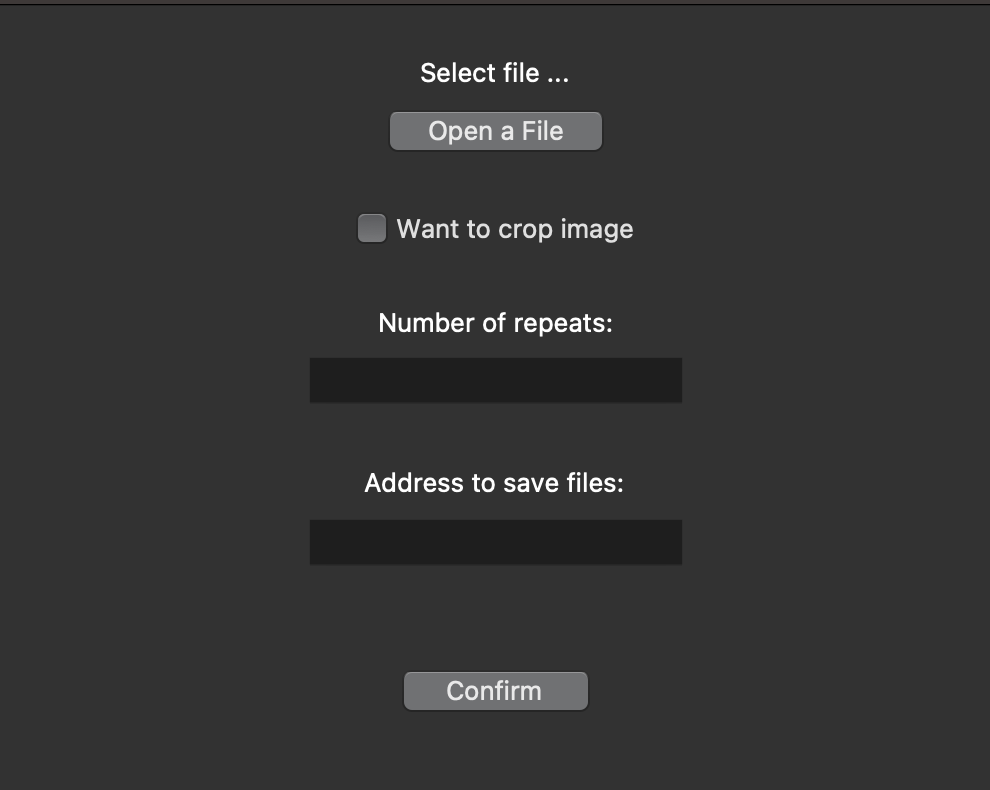
\includegraphics[height=5cm]{GUI-1}\label{gui:f1}}
	\qquad
	\subfloat[رفع واپیچش]{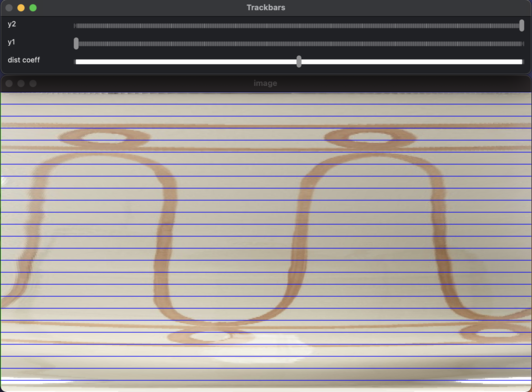
\includegraphics[height=5cm]{GUI-2}\label{gui:f2}}
	\caption{دو رابط کاربری گرافیکی توسعه داده‌شده}
	\label{gui}
\end{figure}






